\documentclass[a4paper, article, oneside, USenglish, IN5460]{memoir}

%% Title page
\usepackage{style/projectfp} 


%% Encoding
\usepackage[utf8]{inputenx} % Source code
\usepackage[T1]{fontenc}    % PDF
\usepackage{float}


%% Fonts and typography
\usepackage{lmodern}           % Latin Modern Roman
\usepackage[scaled]{beramono}  % Bera Mono (Bitstream Vera Sans Mono)
\renewcommand{\sfdefault}{phv} % Helvetica
\usepackage[final]{microtype}  % Improved typography
\renewcommand{\abstractnamefont}{\sffamily\bfseries}                 % Abstract
\renewcommand*{\chaptitlefont}{\Large\bfseries\sffamily\raggedright} % Chapter
\setsecheadstyle{\large\bfseries\sffamily\raggedright}               % Section
\setsubsecheadstyle{\large\bfseries\sffamily\raggedright}            % Subsection
%%\setsubsubsecheadstyle{\normalsize\bfseries\sffamily\raggedright}    % Subsubsection
\setparaheadstyle{\normalsize\bfseries\sffamily\raggedright}         % Paragraph
\setsubparaheadstyle{\normalsize\bfseries\sffamily\raggedright}      % Subparagraph

%% Mathematics
\usepackage{amssymb}   % Extra symbols
\usepackage{amsthm}    % Theorem-like environments
\usepackage{thmtools}  % Theorem-like environments
\usepackage{mathtools} % Fonts and environments for mathematical formuale
\usepackage{mathrsfs}  % Script font with \mathscr{}
% Bibliography
\usepackage[backend=biber,style=numeric-comp]{biblatex}

% Plotting
\usepackage[utf8]{inputenc}
\usepackage{pgfplots}
\DeclareUnicodeCharacter{2212}{−}
\usepgfplotslibrary{groupplots,dateplot}
\usetikzlibrary{patterns,shapes.arrows}
\pgfplotsset{compat=newest}


\usepackage{graphicx}
\usepackage{subcaption}
\usepackage{mwe}

\newlength\figH
\newlength\figW
\setlength{\figH}{8cm}
\setlength{\figW}{12cm}


\DeclareMathOperator*{\min}{\text{\Large minimize}}

\usepackage{optidef}
\usepackage{listings} 


\title{ Wind Energy Forecasting }
\authors{W. Cai, F. Ofstad, E. F. Rørstad}

\addbibresource{bibliography.bib}

\begin{document}

\shorthandoff{}

\projectfrontpage


\chapter{Introduction}
\subsection{linear regression for wind power prediction}
the linear model is defined as $y=wx+b$.
And the residual for observation $i$ is $e_i =y_i -(wx_i+b)$. Thus, linear regression is used to minimize the sum of residual squares, shown as followed:
\begin{equation}
\begin{aligned}
\min_{w,b}\sum_{i=1}^{n} [y_i-(wx_i+b)]^2
\end{aligned}
\end{equation}
\newline


\subsection{K-NN for wind power prediction}
\begin{equation}
\begin{aligned}

\end{aligned}
\end{equation}
\newline

\subsection{SVR for wind power prediction}
\begin{equation}
\begin{aligned}

\end{aligned}
\end{equation}
\newline


\subsection{ANN for wind power prediction}
Each single artificial neuron is defined as the following: 
\begin{equation}
\begin{aligned}
y(x) = f(\sum_{i=1}^{n} w_i*x_i)
\end{aligned}
\end{equation}
where $y(x)$ is the variable for output signal, $x_i$ are variables for input signals, $w_i$ are the weights of corresponding input signals. $f()$ is the activation function of each node. Hidden layers with hidden nodes in between of inputs and the output forms a neural network topology
\newline

\subsection{RNN  for wind power prediction}
\begin{equation}
\begin{aligned}

\end{aligned}
\end{equation}
\newline

\chapter{Question 1}

\section{Comparison of RMSE}
SVR performs the best out of the four models with an RMSE of 0.214, as seen in Table \ref{tab:q1-RMSE-comparison} showing the RMSE value of each of the four models. The ANN is second best with an RMSE of 0.215 and LR/KNN has the same RMSE of 0.217.
\begin{table}[H]
    \centering
    \begin{tabular}{|c|c|c|c|c|} \hline 
        Method & LR & KNN & SVR & ANN\\ \hline 
        RMSE&  0.217&  0.217&  0.214& 0.215\\ \hline
    \end{tabular}
    \label{tab:q1-RMSE-comparison}
\end{table}

\section{Training}
Figure \ref{fig:q1-training-data} illustrates how each models predicts on the training data. It shows how each of the models behave for different inputs. LR is restricted to a linear relationship, but performs okay in this case compared to the other models. It predicts negative power values for low wind speeds with is not correct. KNN regression uses k=1000, and performs similar to LR in terms of RMSE. Difference being all values are legal. SVR seems to outperform the simple ANN even though it does not predict correctly at low wind speed. Furthermore, SVR seems to not predict a lower power output than 0.1. ANN looks pretty good, but is outperformed by SVR, as it does not predicts worse on higher power outputs. KNN and SVR has been optimized with some simple parameter tuning.
\begin{figure}[H]
    \centering
    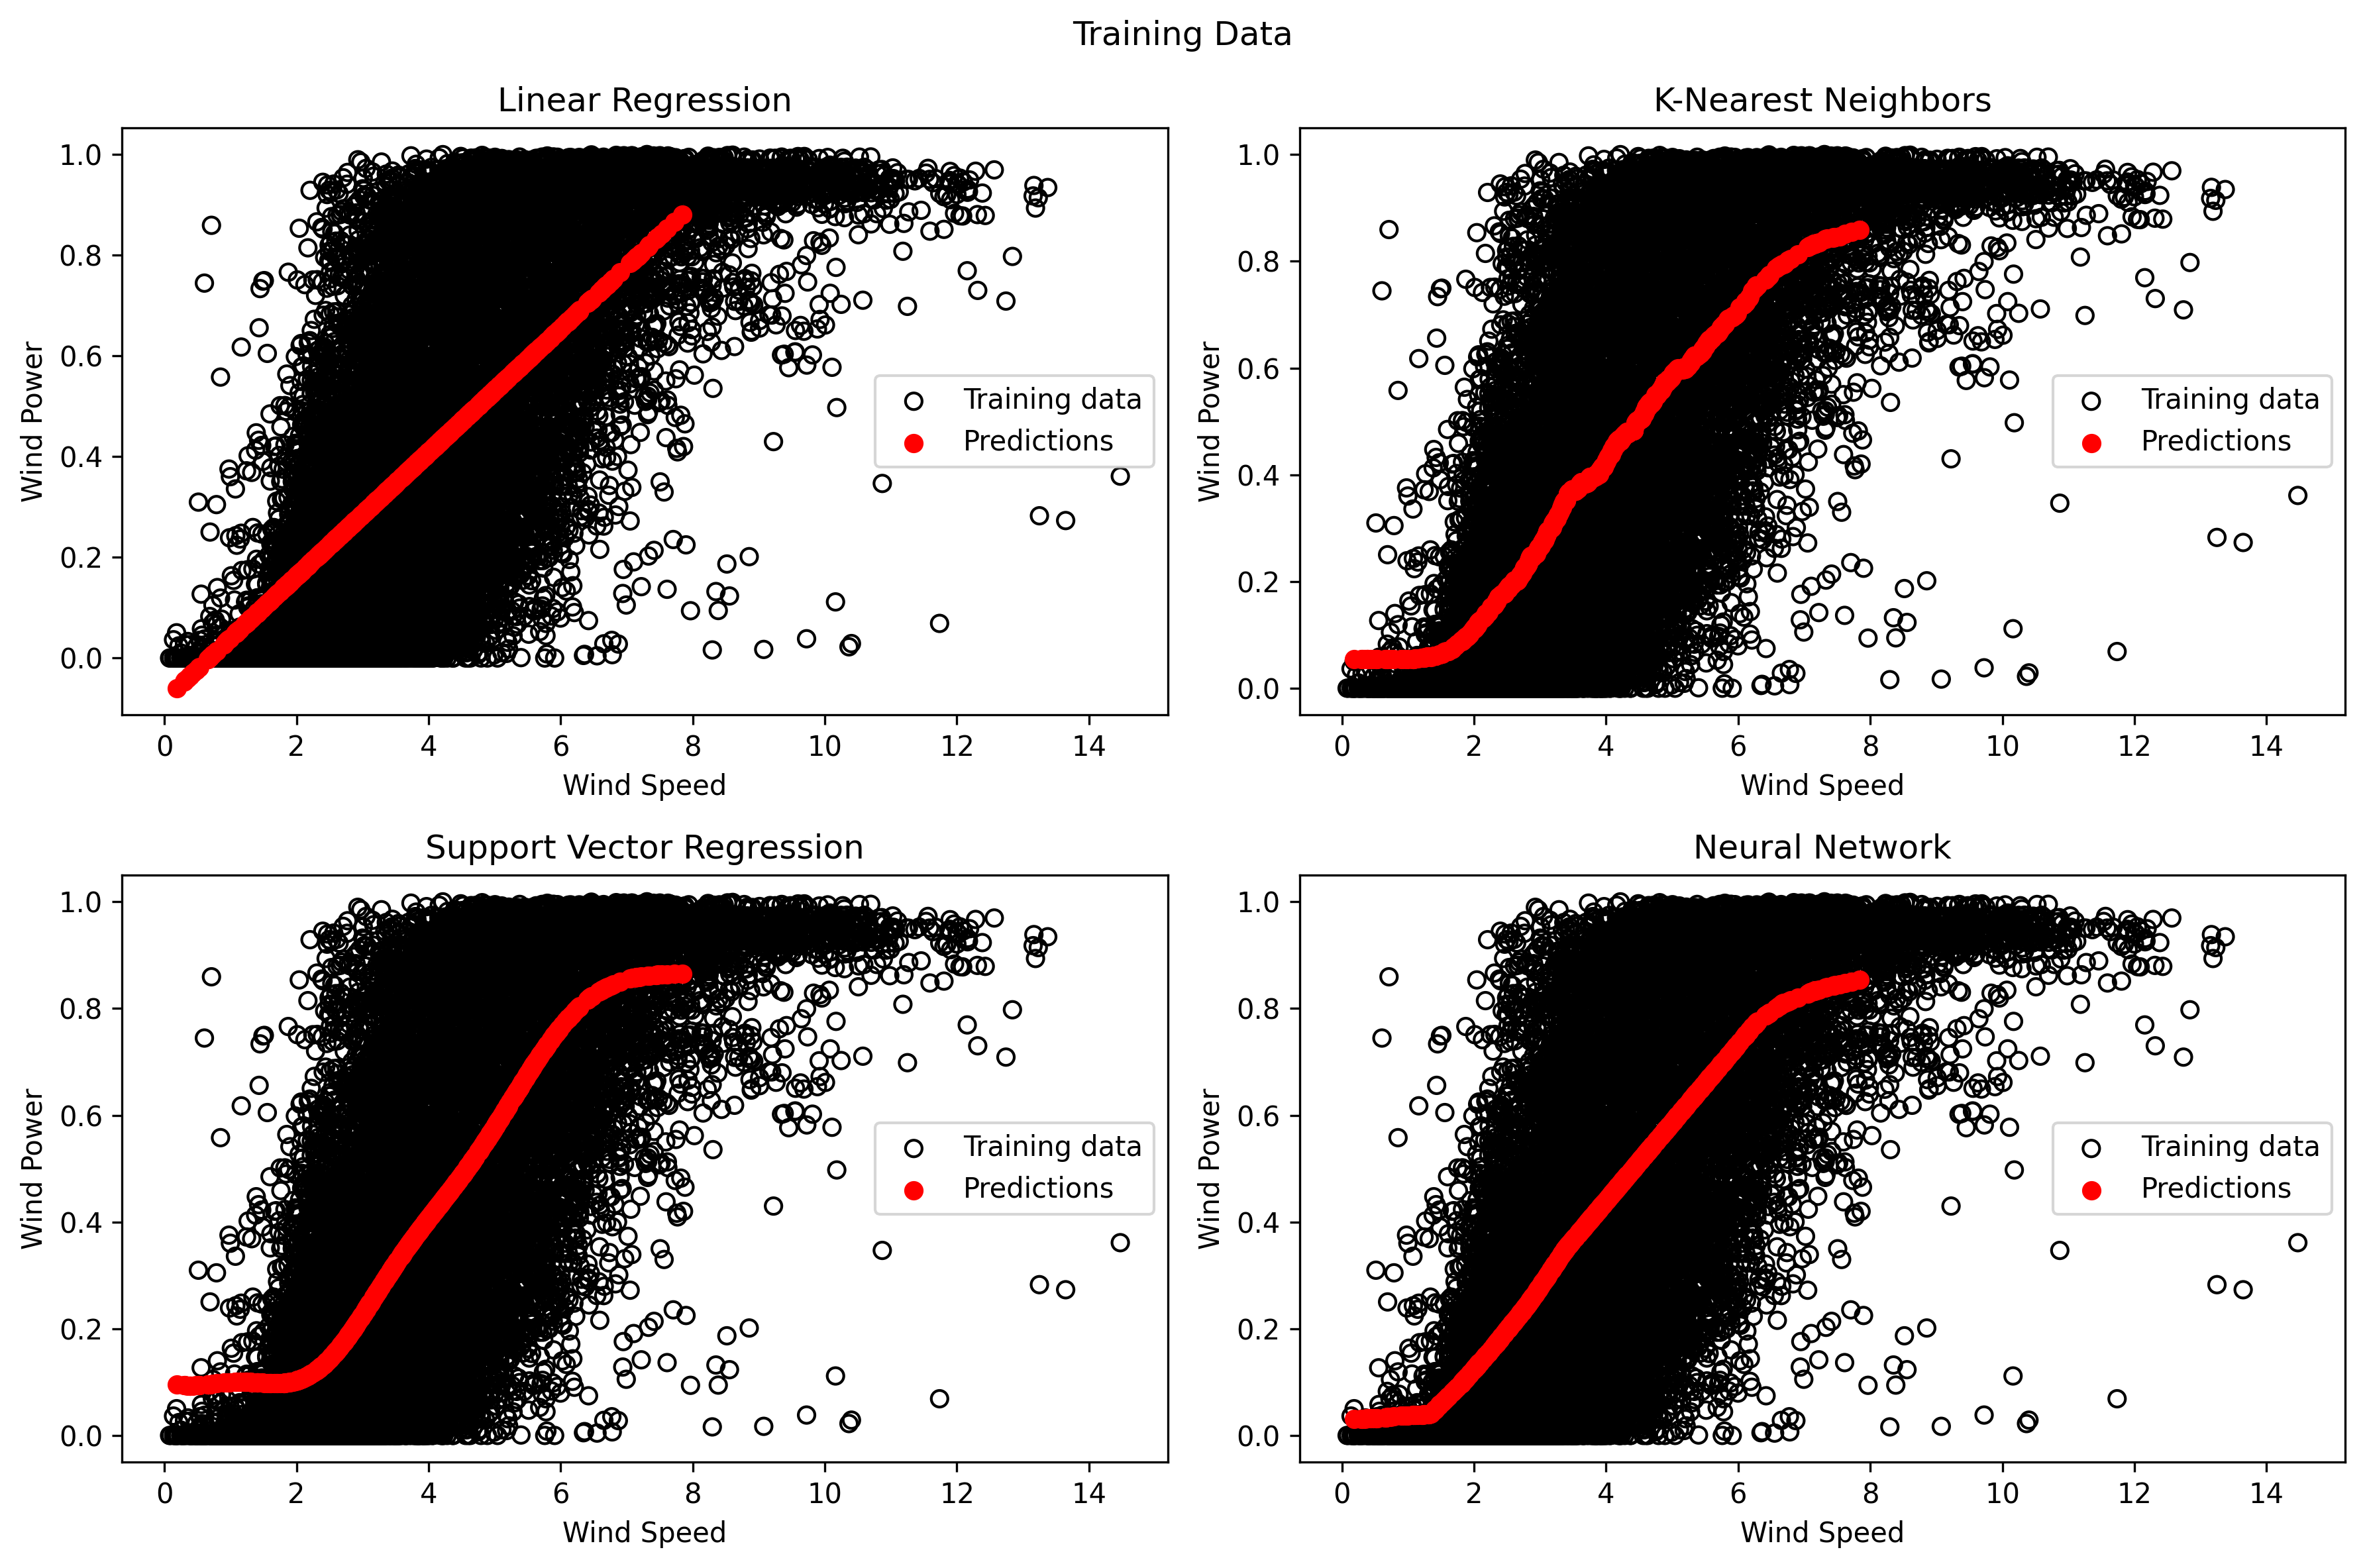
\includegraphics[width=1\linewidth]{fig/q1-ALL-training.png}
    \caption{The figure shows how each model conforms to the training data. It shows what wind power values are predicted for the given wind speed.}
    \label{fig:q1-training-data}
\end{figure}

\section{Forecasts}
Figure \ref{fig:q1-forecast-comparison}  shows the forecasted vs. actual power of the four models. All models performs okay, but they seem to struggle with predicting peak power. LR predicts negative power output in some places, which is wrong. SVR predicts badly for low power compared to the actual power. 
\begin{figure}[H]
    \centering
    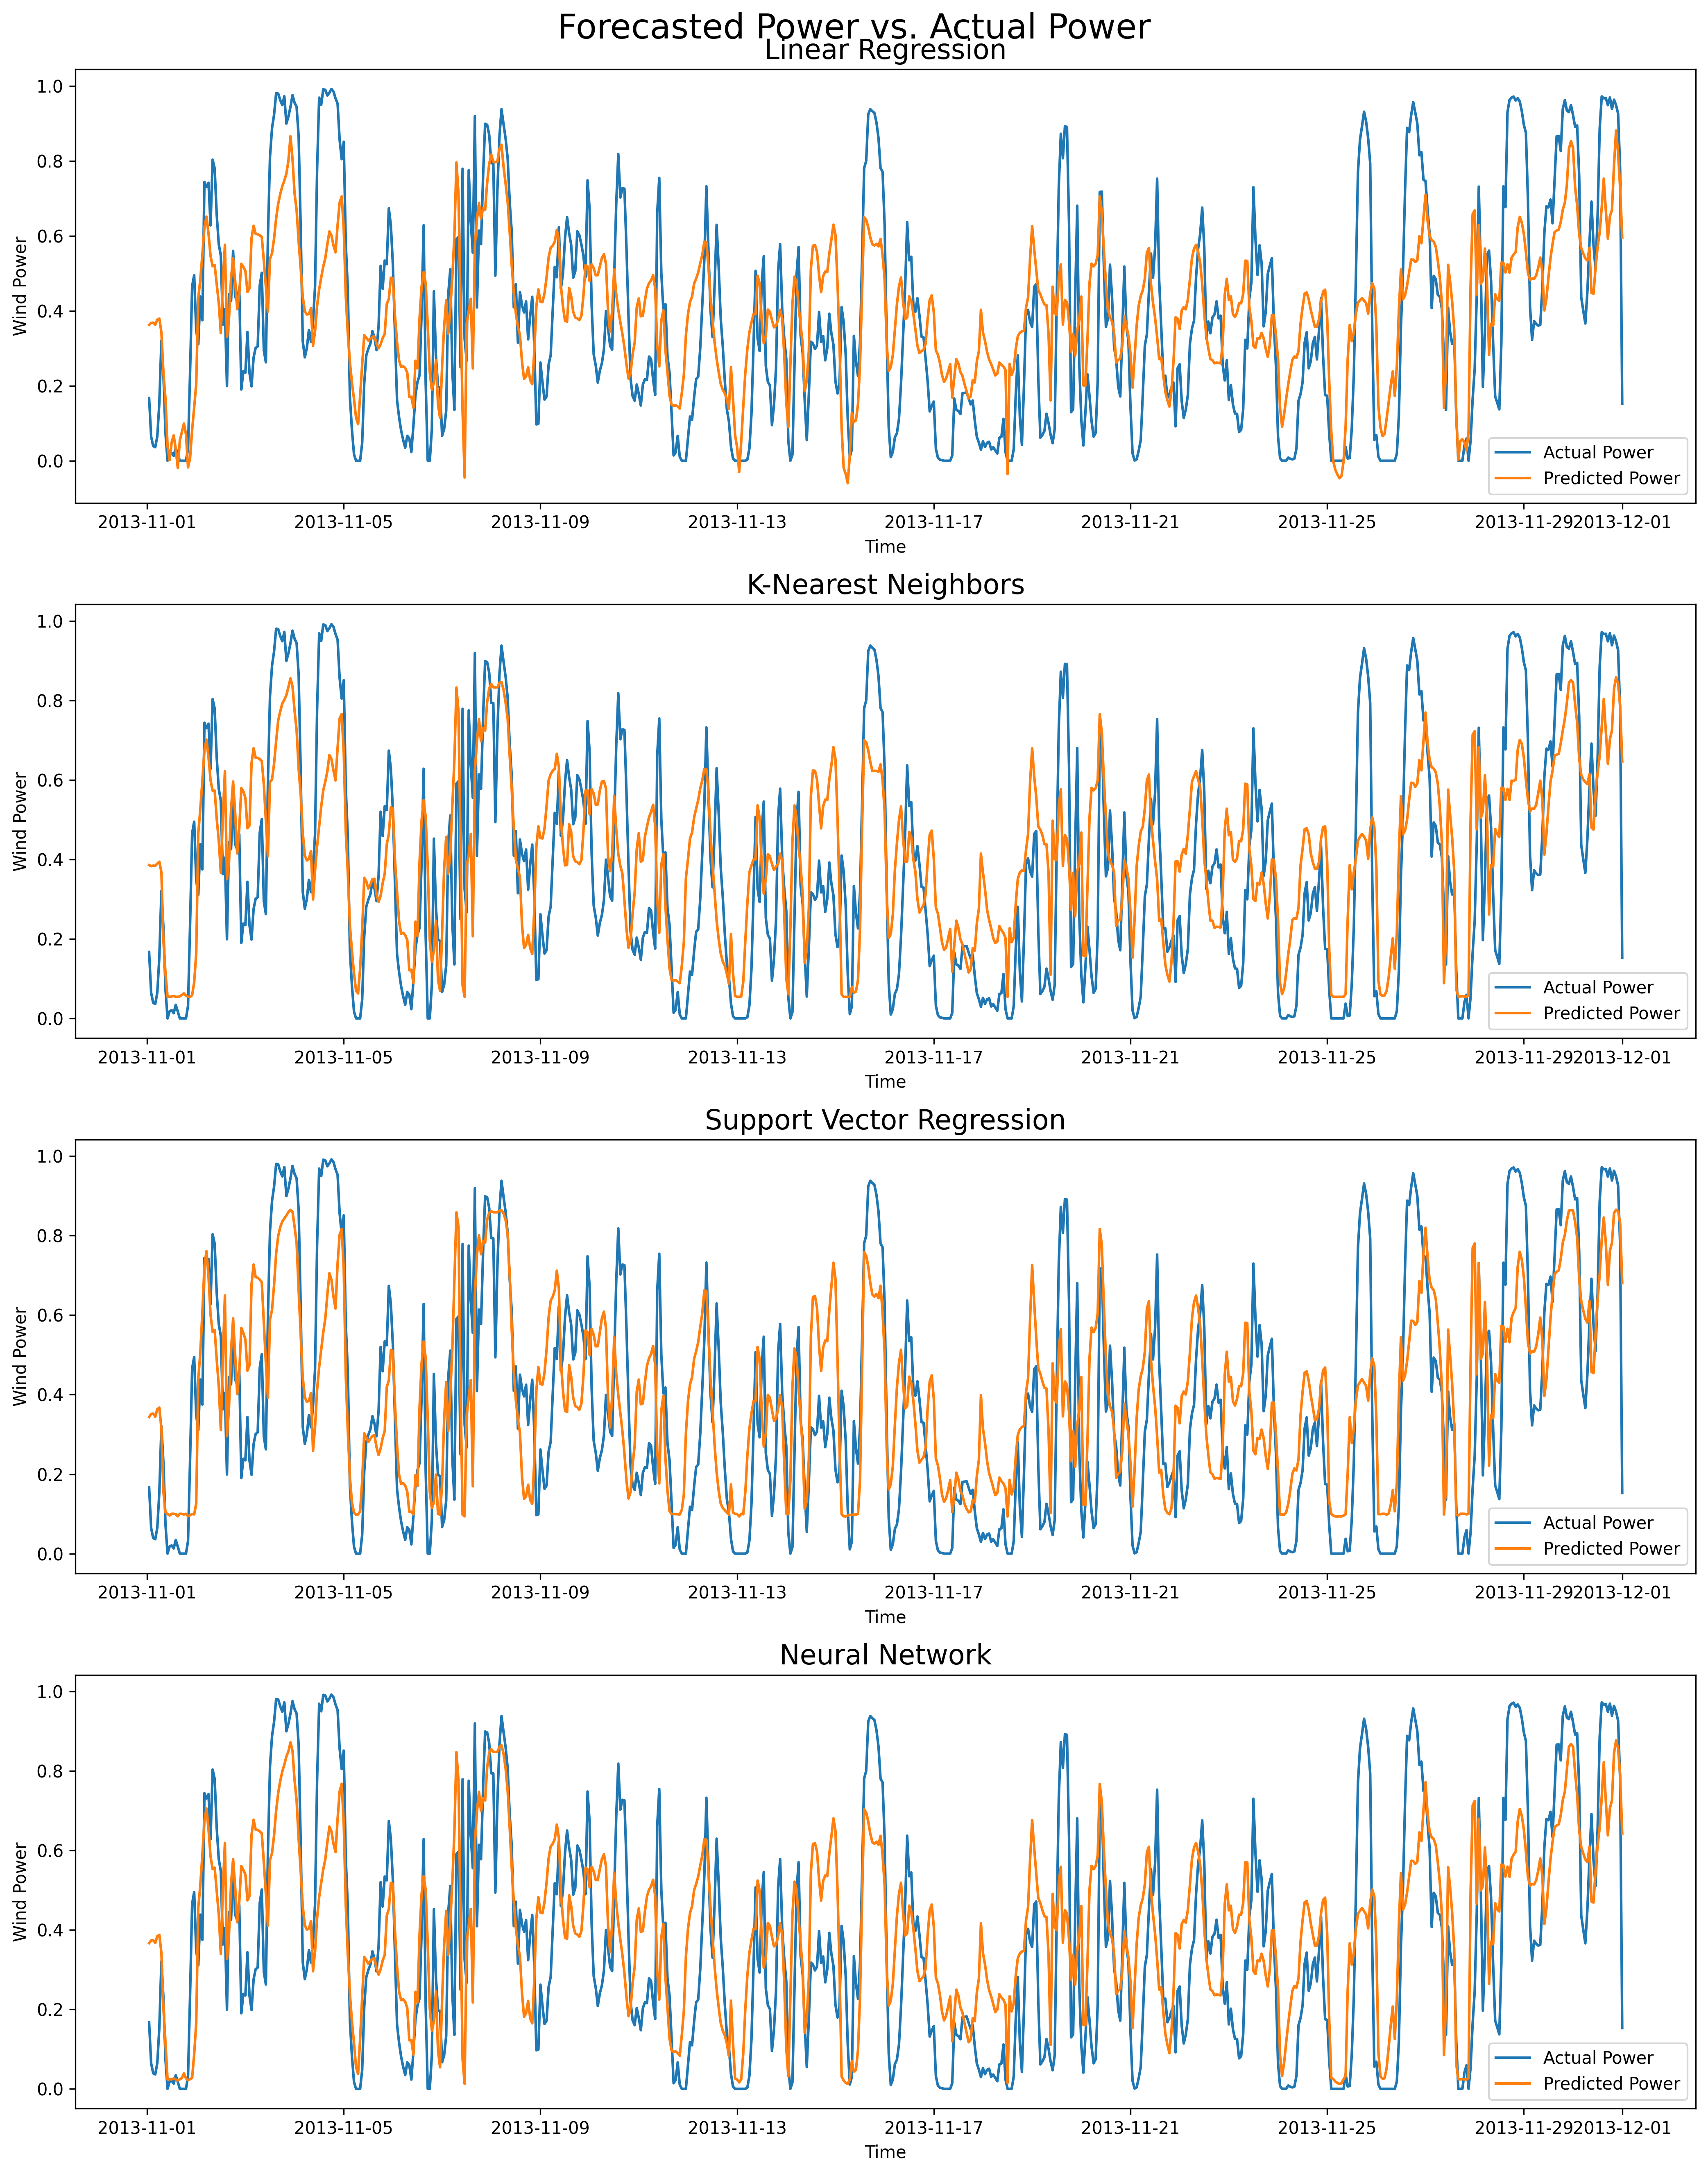
\includegraphics[width=1\linewidth]{fig/q1-ALL-forecast.png}
    \caption{Comparison of forecasts }
    \label{fig:q1-forecast-comparison}
\end{figure}


\chapter{Question 2}


\begin{equation}
\frac{\pi}{2} - \arctan \left(\frac{v_{10}}{u_{10}}\right) \mod 2\pi


\end{equation}


\begin{figure}[H]
    \centering
    \includegraphics[width=1\linewidth]{fig/q2}
    \caption{Comparison of forecasts }
    \label{fig:q2}
\end{figure}


\begin{table}[H]
\begin{tabular}{|l|l|l|}
\hline
Method & LR & MLR  \\ \hline
RMSE   & 0.216  & 0.211    \\ \hline
\end{tabular}
\end{table}


\chapter{Question 3}

LR

SVR

ANN

RNN

-Time series doesn't necessarily provide a linear relationship, make LR not as accurate?

- RNN with its "memory", is the obvious choice for forecasting based on time series.

\begin{table}[H]
\begin{tabular}{|l|l|l|l|l|}
\hline
Method & LR & SVR & ANN & RNN \\ \hline
RMSE   & 0  & 0   & 0   & 0   \\ \hline
\end{tabular}
\end{table}


\chapter{Question 4}

\begin{figure}[H]
\centering
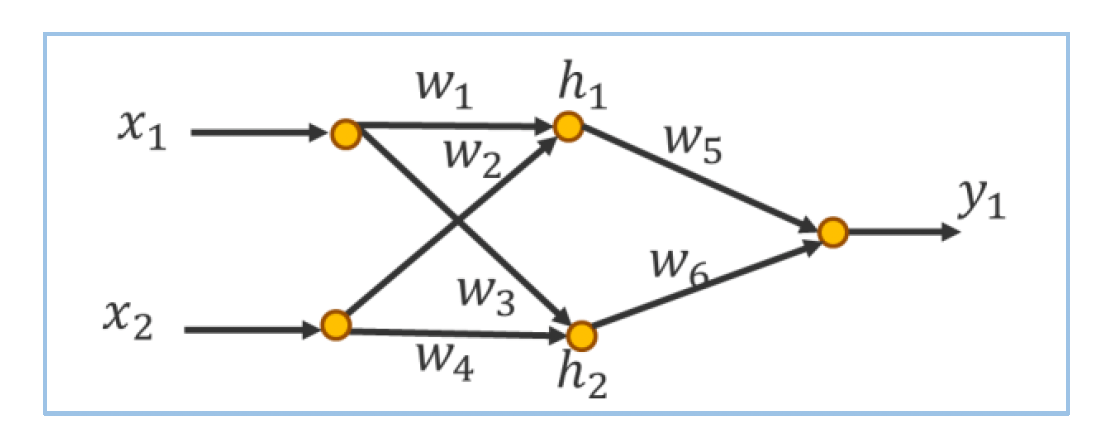
\includegraphics[width=0.8\linewidth]{fig/q4.png}
\caption{\label{fig:q4} \neural network topology}
\end{figure}
{
Given $x_1 = 0.04, x_2 = 0.2, y_1 =0.5,  \alpha = 0.4$, sigmoid activation functions
\newline
\textbf{Initial guess of weights:}
$w_1 = 0.12; 
w_2 = 0.2;
w_3 = 0.11;
w_4 = 0.25;
w_5 = 0.21;
w_6 = 0.3.$ 
% USE PYTHON SHELL TO CALCULATE!!
\newline
\textbf{ Forward: }
$\newline\text{sum}h_1 = w_1*x_1 + w_2*x_2 = 0.044800000000000006 
\newline\text{out}h_1 =sigmoid (\text{sum}h_1) =0.5111981271385566
\newline\text{sum}h_2 = w_3*x_1 + w_4*x_2 =0.054400000000000004
\newline\text{out}h_2 =sigmoid (\text{sum}h_2) =0.5135966470509216
\newline\text{sum}y_1 = w_5*\text{out}h_1 + w_6*\text{out}h_2 = 0.2614306008143733 
\newline\text{out}y_1 =sigmoid (\text{sum}y_1) = 0.5649879325949473$

\newline
\textbf{Error :}

\begin{equation}
\begin{aligned}
\text{E}_{total} &= 
\frac{1}{1}\sum(y_1 -\text{out}y_1)^2 =
0.004223431382965412

\end{aligned}
\end{equation}
\begin{equation}
\begin{aligned}
RMSE = sqrt(\text{E}_{total} ) = 0.06498793259494728
\end{aligned}
\end{equation}
\begin{equation}
\begin{aligned}
\text{E'}_{total}&= 2*(y_1 - \text{out}y_1)*(-1)= 0.12997586518989457
\end{aligned}
\end{equation}

\newline Because $\text{E'}_{total} >0 $, we use gradient descent to update $w_1 \ldots w_6 $



\newline
\textbf{Updating weights :}

for $w_6$ :
\begin{equation}
\begin{aligned}
\frac{\partial \text{E}_{total}  }{\partial w_6} &= 
\frac{\partial \text{E}_{total}}{\partial \text{out}y_1} *\frac{\partial  \text{out}y_1}{\partial \text{sum}y_1}*\frac{\partial \text{sum}y_1}{\partial  w_6}\\
&= [2*(y_1 -\text{out}y_1)*(-1)] * [\text{out}y_1(1-\text{out}y_1)] *\text{out}h_2 \\
& = 0.01640685626590058
\end{aligned}
\end{equation}


\begin{equation}
\begin{aligned}
w^+_6 &= w_6 - \alpha * \frac{\partial \text{E}_{total}  }{\partial w_6} \\
& =  0.29343725749363975
\end{aligned}
\end{equation}


\newline
for $w_5$ :
\begin{equation}
\begin{aligned}
\frac{\partial \text{E}_{total}  }{\partial w_5} &= \frac{\partial \text{E}_{total}}{\partial \text{out}y_1} *\frac{\partial  \text{out}y_1}{\partial \text{sum}y_1}*\frac{\partial \text{sum}y_1}{\partial  w_5}\\
&=[2*(y_1 -\text{out}y_1)*(-1)] * [\text{out}y_1(1-\text{out}y_1)] *\text{out}h_1 \\
& =  0.016330235494174297

\end{aligned}
\end{equation}
\begin{equation}
\begin{aligned}
w^+_5 &= w_5 - \alpha * \frac{\partial \text{E}_{total}  }{\partial w_5} \\
& = 0.20346790580233026
\end{aligned}
\end{equation}


\newline
for $w_4$ :
\begin{equation}
\begin{aligned}
\frac{\partial \text{E}_{total}  }{\partial w_4} &= \frac{\partial \text{E}_{total}}{\partial \text{out}y_1} *\frac{\partial  \text{out}y_1}{\partial \text{sum}y_1}*\frac{\partial \text{sum}y_1}{\partial  w_4} \\
&= \frac{\partial \text{E}_{total}}{\partial \text{out}y_1} *\frac{\partial  \text{out}y_1}{\partial \text{sum}y_1}*\frac{\partial ( w_5*\text{out}h_1 + w_6*\text{out}h_2 )} {\partial w_4} \\
&= \frac{\partial \text{E}_{total}}{\partial \text{out}y_1} * \frac{\partial \text{out}y_1}{\partial \text{sum}y_1} *{w_6}* \frac{\partial ( \text{out}h_2 )} {\partial w_4}\\
&= \frac{\partial \text{E}_{total}}{\partial \text{out}y_1} * \frac{\partial \text{out}y_1}{\partial \text{sum}y_1} *{w_6}* \frac{\partial ( \text{out}h_2 )}{\partial \text{sum}h_2} * \frac{\partial ( \text{sum}h_2)}{\partial w_4}\\
&= \frac{\partial \text{E}_{total}}{\partial \text{out}y_1} * \frac{\partial \text{out}y_1}{\partial \text{sum}y_1} *{w_6}* \frac{\partial ( \text{out}h_2 )}{\partial \text{sum}h_2} * \frac{\partial ( w_3*x_1 + w_4*x_2)}{\partial w_4}\\
&= \frac{\partial \text{E}_{total}}{\partial \text{out}y_1} * \frac{\partial \text{out}y_1}{\partial \text{sum}y_1} *{w_6}* \frac{\partial ( \text{out}h_2 )}{\partial \text{sum}h_2} *  {x_2}\\
&= [2*(y_1 -\text{out}y_1)*(-1)] * [\text{out}y_1(1-\text{out}y_1)] *{w_6}* [\text{out}h_2 (1-\text{out}h_2)]*  {x_2}\\
& = 0.0004788209939452584

 \end{aligned}
\end{equation}
\begin{equation}
\begin{aligned}
w^+_4 &= w_4 - \alpha * \frac{\partial \text{E}_{total}  }{\partial w_4} \\
& = 0.2498084716024219
\end{aligned}
\end{equation}

\newline
for $w_3$ :
\begin{equation}
\begin{aligned}
\frac{\partial \text{E}_{total}  }{\partial w_3} &= \frac{\partial \text{E}_{total}}{\partial \text{out}y_1} *\frac{\partial  \text{out}y_1}{\partial \text{sum}y_1}*\frac{\partial \text{sum}y_1}{\partial  w_3} \\
&= \frac{\partial \text{E}_{total}}{\partial \text{out}y_1} *\frac{\partial  \text{out}y_1}{\partial \text{sum}y_1}*\frac{\partial ( w_5*\text{out}h_1 + w_6*\text{out}h_2 )} {\partial w_3} \\
&= \frac{\partial \text{E}_{total}}{\partial \text{out}y_1} * \frac{\partial \text{out}y_1}{\partial \text{sum}y_1} *{w_6}* \frac{\partial ( \text{out}h_2 )} {\partial w_3}\\
&= \frac{\partial \text{E}_{total}}{\partial \text{out}y_1} * \frac{\partial \text{out}y_1}{\partial \text{sum}y_1} *{w_6}* \frac{\partial ( \text{out}h_2 )}{\partial \text{sum}h_2} * \frac{\partial ( \text{sum}h_2)}{\partial w_3}\\
&= \frac{\partial \text{E}_{total}}{\partial \text{out}y_1} * \frac{\partial \text{out}y_1}{\partial \text{sum}y_1} *{w_6}* \frac{\partial ( \text{out}h_2 )}{\partial \text{sum}h_2} * \frac{\partial ( w_3*x_1 + w_4*x_2)}{\partial w_3}\\
&= \frac{\partial \text{E}_{total}}{\partial \text{out}y_1} * \frac{\partial \text{out}y_1}{\partial \text{sum}y_1} *{w_6}* \frac{\partial ( \text{out}h_2 )}{\partial \text{sum}h_2} *  {x_1}\\
&= [2*(y_1 -\text{out}y_1)*(-1)] * [\text{out}y_1(1-\text{out}y_1)] *{w_6}* [\text{out}h_2 (1-\text{out}h_2)]*  {x_1}\\
& = 9.576419878905167e-5
\end{aligned}
\end{equation}
\begin{equation}
\begin{aligned}
w^+_3 &= w_3 - \alpha * \frac{\partial \text{E}_{total}  }{\partial w_3} \\
& =  0.1099616943204843
\end{aligned}
\end{equation}

\newline
for $w_2$ :
\begin{equation}
\begin{aligned}
\frac{\partial \text{E}_{total}  }{\partial w_2} &= \frac{\partial \text{E}_{total}}{\partial \text{out}y_1} *\frac{\partial  \text{out}y_1}{\partial \text{sum}y_1}*\frac{\partial \text{sum}y_1}{\partial  w_2} \\
&= \frac{\partial \text{E}_{total}}{\partial \text{out}y_1} *\frac{\partial  \text{out}y_1}{\partial \text{sum}y_1}*\frac{\partial ( w_5*\text{out}h_1 + w_6*\text{out}h_2 )} {\partial w_2} \\
&= \frac{\partial \text{E}_{total}}{\partial \text{out}y_1} * \frac{\partial \text{out}y_1}{\partial \text{sum}y_1} *{w_5}* \frac{\partial ( \text{out}h_1 )} {\partial w_2}\\
&= \frac{\partial \text{E}_{total}}{\partial \text{out}y_1} * \frac{\partial \text{out}y_1}{\partial \text{sum}y_1} *{w_5}* \frac{\partial ( \text{out}h_1 )}{\partial \text{sum}h_1} * \frac{\partial ( \text{sum}h_1)}{\partial w_2}\\
&= \frac{\partial \text{E}_{total}}{\partial \text{out}y_1} * \frac{\partial \text{out}y_1}{\partial \text{sum}y_1} *{w_5}* \frac{\partial ( \text{out}h_1 )}{\partial \text{sum}h_1} * \frac{\partial ( w_1*x_1 + w_2*x_2)}{\partial w_2}\\
&= \frac{\partial \text{E}_{total}}{\partial \text{out}y_1} * \frac{\partial \text{out}y_1}{\partial \text{sum}y_1} *{w_5}* \frac{\partial ( \text{out}h_1 )}{\partial \text{sum}h_1} *  {x_2}\\
&= [2*(y_1 -\text{out}y_1)*(-1)] * [\text{out}y_1(1-\text{out}y_1)] *{w_5}* [\text{out}h_1 (1-\text{out}h_1)]*  {x_2}\\
& = 0.0003352544871404742
\end{aligned}
\end{equation}
\begin{equation}
\begin{aligned}
w^+_2 &= w_2 - \alpha * \frac{\partial \text{E}_{total}  }{\partial w_2} \\
& = 0.19986589820514383
\end{aligned}
\end{equation}


\newline
for $w_1$ :
\begin{equation}
\begin{aligned}
\frac{\partial \text{E}_{total}  }{\partial w_1} &= \frac{\partial \text{E}_{total}}{\partial \text{out}y_1} *\frac{\partial  \text{out}y_1}{\partial \text{sum}y_1}*\frac{\partial \text{sum}y_1}{\partial  w_1} \\
&= \frac{\partial \text{E}_{total}}{\partial \text{out}y_1} *\frac{\partial  \text{out}y_1}{\partial \text{sum}y_1}*\frac{\partial ( w_5*\text{out}h_1 + w_6*\text{out}h_2 )} {\partial w_1} \\
&= \frac{\partial \text{E}_{total}}{\partial \text{out}y_1} * \frac{\partial \text{out}y_1}{\partial \text{sum}y_1} *{w_5}* \frac{\partial ( \text{out}h_1 )} {\partial w_1}\\
&= \frac{\partial \text{E}_{total}}{\partial \text{out}y_1} * \frac{\partial \text{out}y_1}{\partial \text{sum}y_1} *{w_5}* \frac{\partial ( \text{out}h_1 )}{\partial \text{sum}h_1} * \frac{\partial ( \text{sum}h_1)}{\partial w_1}\\
&= \frac{\partial \text{E}_{total}}{\partial \text{out}y_1} * \frac{\partial \text{out}y_1}{\partial \text{sum}y_1} *{w_5}* \frac{\partial ( \text{out}h_1 )}{\partial \text{sum}h_1} * \frac{\partial ( w_1*x_1 + w_2*x_2)}{\partial w_1}\\
&= \frac{\partial \text{E}_{total}}{\partial \text{out}y_1} * \frac{\partial \text{out}y_1}{\partial \text{sum}y_1} *{w_5}* \frac{\partial ( \text{out}h_1 )}{\partial \text{sum}h_1} *  {x_1}\\
&= [2*(y_1 -\text{out}y_1)*(-1)] * [\text{out}y_1(1-\text{out}y_1)] *{w_5}* [\text{out}h_1 (1-\text{out}h_1)]*  {x_1}\\
& = 6.705089742809484e-5
\end{aligned}
\end{equation}
\begin{equation}
\begin{aligned}
w^+_1 &= w_1 - \alpha * \frac{\partial \text{E}_{total}  }{\partial w_1} \\
& = 
0.11997317964102876
\end{aligned}
\end{equation}

\newline
We set $d= 0.0001$ as the threshold for the difference between the error in a round and the error in the previous round.  Our training program gives out the finalized model with updated weights and RMSE:
\newline
$
\newline w_1=0.11956974287617168, , 
\newline w_2=0.1978487143808587, , 
\newline w_3=0.1091489032411234,  ,
\newline w_4=0.24574451620561713, , 
\newline w_5=-0.030695635344251397, ,
\newline w_6=0.058200264079797115, ,
\newline \text{RMSE}=0.0036431398381499003
$


\begin{table}[htbp] % Place the table here, at the top, bottom, or on a separate page (h: here, t: top, b: bottom, p: separate page)
    \centering % Center the table horizontally
    \caption{RMSE Changes in the Training Process } % Table caption
    \label{tab:example} % Table label for referencing
    \begin{tabular}{|c|c|} % Table columns and alignment (c: centered, l: left-aligned, r: right-aligned)
        \hline % Horizontal line
        Training Round Series Number & RMSE Value \\ % Table header row
        \hline % Horizontal line
        The initial round & 0.06498793259494728 \\ % Table content row 1
        $1^{st}$ round after updating weights & 0.06333704131057094 \\ % Table content row 2
        $2^{nd}$ round after updating weights &  0.061725451658177444 \\ % Table content row 3
        $3^{rd}$ round after updating weights & 0.06015242252806485 \\ % Table content row 3
        $4^{th}$ round after updating weights & 0.05861721211584259 \\ % Table content row 3
        $5^{th}$ round after updating weights & 0.057119079240626425 \\ % Table content row 3
        $6^{th}$ round after updating weights & 0.05565728455656549 \\ % Table content row 3
        $7^{th}$ round after updating weights & 0.05423109166303686 \\ % Table content row 3
        $8^{th}$ round after updating weights &  0.05283976811880964 \\ % Table content row 3
        $9^{th}$ round after updating weights & 0.0514825863654198\\ % Table content row 3
        $10^{th}$ round after updating weights & 0.050158824564894955 \\ % Table content row 3
        Final round when updating stops & 0.0036431398381499003 \\ % Table content row 3
        
        
        \hline % Horizontal line
    \end{tabular}
\end{table}

\color{blue}To use neural network with all features provided, we build a ANN model with the following topology: v10,u10 to calculate wind direction at 10 meter as input of $x_1$, wind speed at 10 meter as $x_2$. v100 and u100 to calculate wind direction at 100 meter as input of $x_3$,  wind speed at 100 meter as $x_4$, shown as Figure. \ref{fig:q41}.
The angular parameter $z$ is calculated based on the following formula: 
$z = arctan(V/U)$, where  
$V$ is  meridional component and $U$ is zonal component

\color{red}{write program of this model , and a paragraph to explan the predicted values vs. actual measurements }
\begin{figure}
\centering
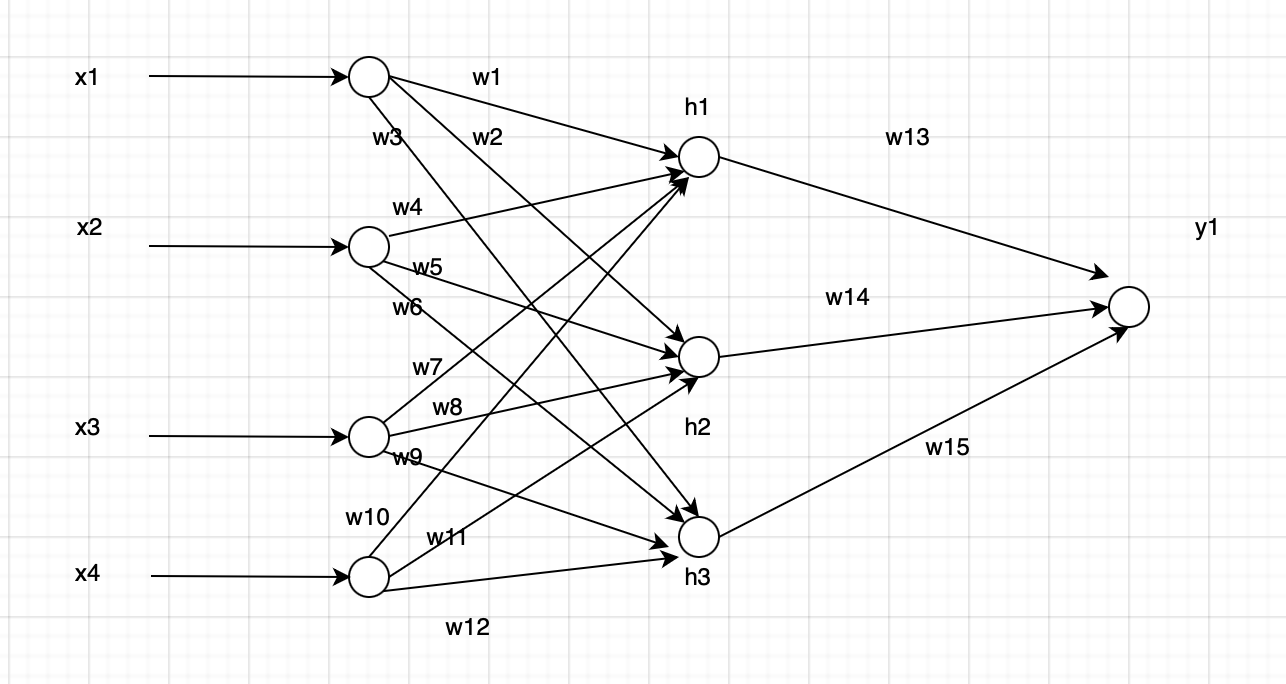
\includegraphics[width=0.8\linewidth]{fig/q41.png}
\caption{\label{fig:q41} \neural ANN Topology for All Features}
\end{figure}

}


\printbibliography{reference}
\bibitem[1]{https://amt.copernicus.org/articles/15/3465/2022/}


\end{document}

